\documentclass{mcmthesis}
\mcmsetup{CTeX = false,   % 使用 CTeX 套装时,设置为 true
        tcn = 011, problem = B,
        sheet = true, titleinsheet = true, keywordsinsheet = true,
        titlepage = true}
\usepackage{palatino}
\usepackage{mwe}
\usepackage{graphicx}
\usepackage{subfig}
\usepackage{subcaption}
\usepackage{float}
\usepackage{multirow}
\usepackage{indentfirst}
\usepackage{gensymb}
\usepackage[ruled,lined,commentsnumbered]{algorithm2e}
\usepackage{geometry}
\usepackage{pdfpages}
\usepackage{array}
\geometry{left=2cm,right=2cm,top=2cm,bottom=2cm} %%页边距

\begin{document}

\linespread{0.6} %%行间距
\setlength{\parskip}{0.5\baselineskip} %%段间距

\section{Route Selection Model}
\subsection{Model}
In this section, we firstly introduce concepts related to a route map. Then we analyze factors that could affect the quality of a route map, and define the cost function for a given route map. Finally, we devise an algorithm that could transform samples in primary sample space to a route map, which could be used to find optimal solutions with Simulated Annealing.

\subsubsection{Route Map Concepts}
Based on destinations selected in previous section, we can plan the routes for all the buses. At the very beginning of this section, we'd like to define the concept of a route map. In our model, a route map is a tree data structure\cite{TreeStructure}, as presented in Figure \ref{roadmap_demo}. The root node of the tree represents the airport, so we denote it as $V_A$. All the nodes on the tree, except root node and leaf nodes, have only one parent node and one child node. A route $R_i$ is the path from root node to $i$th leave node. Assume that we plan to have $N_r$ routes that depart from the airport, then we have $N_r$ leave nodes in the road map, correspondingly. For each route $R_i$, every vertex $V_{i, j}$(or node in the context of a tree) on the route represents a station, where $j$ is the index of the vertex on that route. Obviously, the airport vertex is the starting vertex of all routes, so $V_{i, 0} = V_A$. Every edge $E_{i, j}$ represents the journey from $V_{i, j-1}$ to $V_{i,j}$. 

\begin{figure}[htbp]
	\centering
	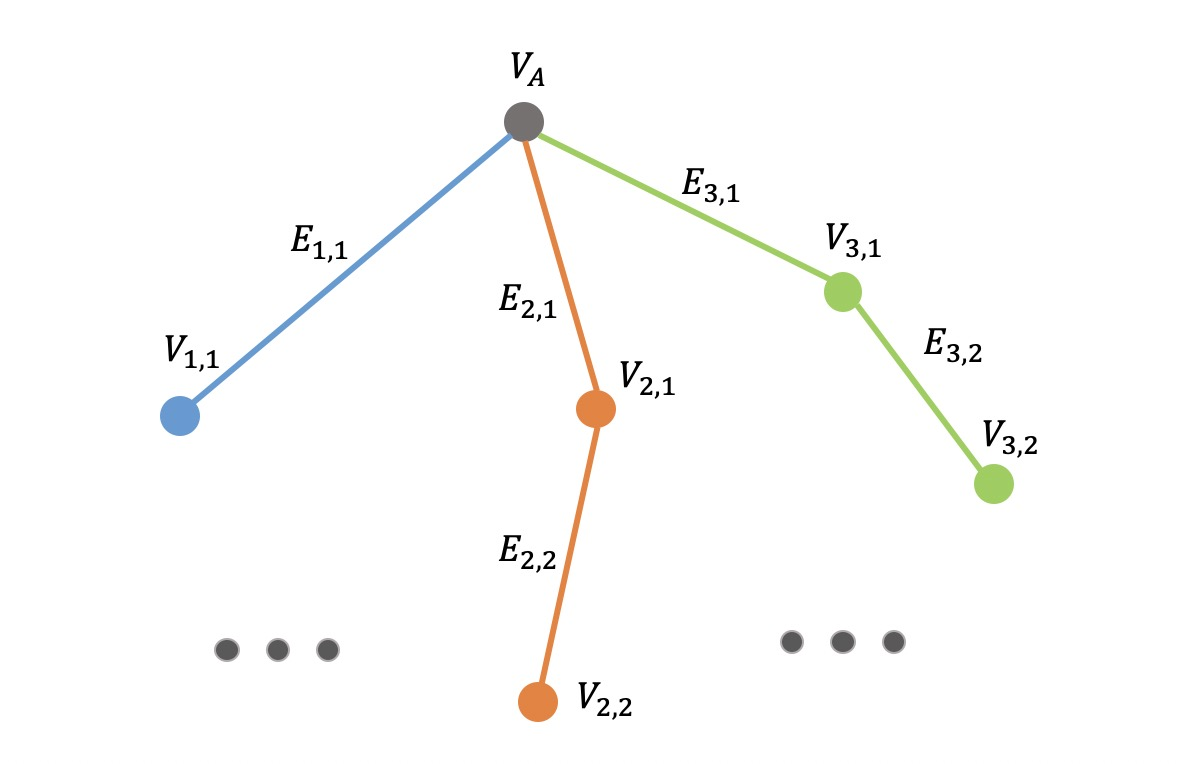
\includegraphics[width=14cm]{figures/routedemo.jpg}
	\caption{Demonstration of a road map}
    \label{roadmap_demo}
\end{figure}

All the vertices and edges on the route map all have certain information related to it. For each vertex $V_{i, j}$, we have its location $\rho_{i, j}$ and population density $p_{i, j} = P(\rho_{x,i,j}, \rho_{y,i,j})$. For each edge $E_{i, j}$, we have its taxicab metric\cite{ManhatDist}: 
\begin{equation}
d_{i,j} = |\rho_{x,i,j-1} - \rho_{x,i,j}| + |\rho_{y,i,j-1} - \rho_{y,i,j}| 
\end{equation}
Also, we have its average traffic density along a taxicab path $l_{i,j}$ from $\rho_{i,j-1}$ to $\rho_{i, j}$:
\begin{equation}
t_{i,j} = \frac{\int_{l_{1,i,j}} T(\rho_{x}, \rho_{y})\mathrm{d}l}{d_{i,j}}
\label{traf_den}
\end{equation}
However, it's impossible to compute the value of Equation \ref{traf_den}, since it depends on path of integration. Here we provide a discrete method to estimate this integral on one of the path. We divide path $l_{i,j}$ from $\rho_{i,j-1}$ to $\rho_{i, j}$ to $N_{l_s}$ segments $l_{s, i, j} = l_{i,j}/N_{l_s}$. Then Equation \ref{traf_den} can be estimated as
\begin{equation}
t_{i,j} \approx \frac{1}{d_{i,j}}\sum\limits_{k=0}^{N_{l_s}-1} T(\rho_{x,i,j-1}+k\cdot l_{sx,i,j}, \rho_{y,i,j-1}+k\cdot l_{sy,i,j})
\label{traf_approx}
\end{equation}
With Equation \ref{traf_approx}, $t_{i,j}$ can be easily computed through discrete samples of $T(x,y)$. 

\subsubsection{Route Cost Function}
With structure and related properties of a route map defined, we can now move on to the cost function part. There are many factors that could affect the quality of a route map. Some of them can be easily quantified, while others are not. The strategy of our model is that we take factors whose data is easily accessible into account of our cost function, and put others aside. We use these factors considered to evaluate our cost function, find the optimal result of such function, and revise the result with human intervention. To be mentioned, the last step, i.e. human intervention should only impose subtle influence to the final result, while design and  optimization of the algorithm should be greatly emphasized.

Among all the factors, we choose three of them: distance of journey $d_{i,j}$, traffic density $t_{i,j}$ and population density $p_{i,j}$. The lower the cost of a route map is, the better the Now we analyze their specific relationship, respectively. 

\subsection{Implementation}

\end{document}


